%%%%%%%%%%%%%%%%%%%%%%%%%%%%%%%%%%%%%%%%%%%%%%%%%%%%%%%%%%%%%%%%%%%%%%%%%%%%%%%%
% FUENTE
%%%%%%%%%%%%%%%%%%%%%%%%%%%%%%%%%%%%%%%%%%%%%%%%%%%%%%%%%%%%%%%%%%%%%%%%%%%%%%%%

% Plantilla creada por Eduardo Mosqueira Rey a partir de un original de
% Rational Software Corporation

%%%%%%%%%%%%%%%%%%%%%%%%%%%%%%%%%%%%%%%%%%%%%%%%%%%%%%%%%%%%%%%%%%%%%%%%%%%%%%%%
% CONFIGURACIÓN TEXSTUDIO DEL CORRECTOR ORTOGRÁFICO
%%%%%%%%%%%%%%%%%%%%%%%%%%%%%%%%%%%%%%%%%%%%%%%%%%%%%%%%%%%%%%%%%%%%%%%%%%%%%%%%

% !TeX spellcheck = es_ES
% Usar el lenguaje es_ES para la corrección en castellano

%%%%%%%%%%%%%%%%%%%%%%%%%%%%%%%%%%%%%%%%%%%%%%%%%%%%%%%%%%%%%%%%%%%%%%%%%%%%%%%%
% TIPO DE DOCUMENTO Y PAQUETES
%%%%%%%%%%%%%%%%%%%%%%%%%%%%%%%%%%%%%%%%%%%%%%%%%%%%%%%%%%%%%%%%%%%%%%%%%%%%%%%%

\documentclass[12pt, a4paper, titlepage]{article}

\usepackage[spanish]{babel} % Soporte multilenguaje para LaTeX.
\usepackage[a4paper, top=2.5cm, bottom=2.5cm, left=2.5cm, right=2.5cm]{geometry} % Interfaz flexible para definir las dimensiones del documento
\usepackage[utf8]{inputenc} % Aceptar diferentes tipos de codificación de caracteres de entrada (en este caso usamos la codificación Unicode UTF-8)
\usepackage{graphicx} % Soporte aumentado para gráficos 
\usepackage{color} % Para usar colores
\usepackage{hyperref} % Para manejar referencias cruzadas. P.ej. añadir hiperenlaces al índice


\begin{document}
	
	%%%%%%%%%%%%%%%%%%%%%%%%%%%%%%%%%%%%%%%%%%%%%%%%%%%%%%%%%%%%%%%%%%%%%%%%%%%%%%%%
	% PORTADA
	%%%%%%%%%%%%%%%%%%%%%%%%%%%%%%%%%%%%%%%%%%%%%%%%%%%%%%%%%%%%%%%%%%%%%%%%%%%%%%%%
	
	\begin{titlepage}
		
		
\includegraphics[width=15cm]{Imagenes/Simbolo_logo_UDC.png}
		
		% Lista de tamaños: \Huge, \huge, \LARGE, \Large, \large, \small, \footnotesize, \tiny
		\vspace{6cm}
		
		\begin{flushright}
			
			\LARGE{\textbf{Monitorización de pruebas}}
			
			\large{\textbf{VVS}}
		\end{flushright}
		
		\vspace{3cm}
		\begin{center}
			\large{\textbf{Historial de revisiones}}
			
			\begin{tabular}{ | p{3cm} | p{2cm} | p{4cm} | p{6cm} |}
				\hline
				\textbf{Fecha} & \textbf{Versión} & \textbf{Descripción} & \textbf{Autores} \\ \hline
				16/12/2015 &  1.0 &  Ejercicio de refactorización & Xoán Andreu Barro Torres \newline F. Javier Moure López \newline Emma Oitavén Carracedo \\ \hline
			\end{tabular}
		\end{center}
		
	\end{titlepage}
	\clearpage
	
	%%%%%%%%%%%%%%%%%%%%%%%%%%%%%%%%%%%%%%%%%%%%%%%%%%%%%%%%%%%%%%%%%%%%%%%%%%%%%%%%
	% INDICE
	%%%%%%%%%%%%%%%%%%%%%%%%%%%%%%%%%%%%%%%%%%%%%%%%%%%%%%%%%%%%%%%%%%%%%%%%%%%%%%%%
	
	\tableofcontents
	\newpage
	
	%%%%%%%%%%%%%%%%%%%%%%%%%%%%%%%%%%%%%%%%%%%%%%%%%%%%%%%%%%%%%%%%%%%%%%%%%%%%%%%%
	\section{Contexto}
	
	Este documento hace referencia a las pruebas realizadas sobre el proyecto de la asignatura VVS llamado Spoticopy\footnote{https://github.com/andreu-barro/VVS} encontrado en el repositorio de GitHub. Dicha aplicación simula el comportamiento de una aplicación de música. El enunciado de la funcionalidad es el siguiente:\\
	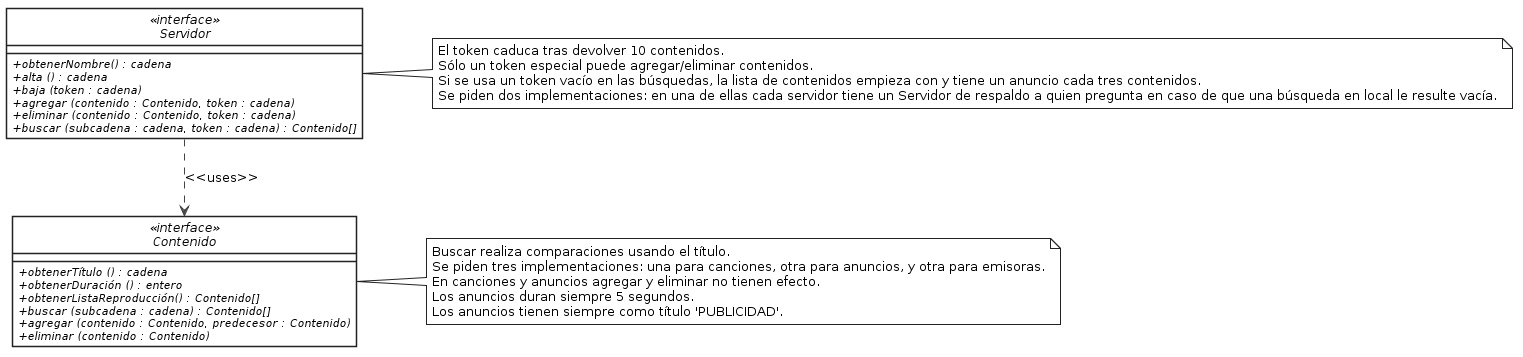
\includegraphics[width=18cm]{Imagenes/DiagramaSimple.png}\\
	A partir de dicho diagrama obtuvimos la siguiente relación de clases:\\
		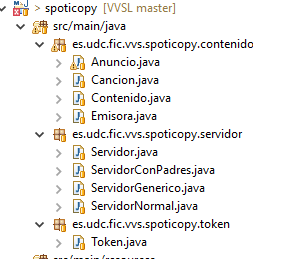
\includegraphics[width=8cm]{Imagenes/Clases.png} \\
	El paquete contenido tienen siempre un nombre, una duración y una lista de reproducción. Son las unidades funcionales con las que funcionará nuestro servidor.
	El paquete servidor es el que utiliza el paquete contenido para simular el funcionamiento de una aplicación que reproduce música. Distinguiremos ServidorGenerico que contiene el comportamiento genérico de un servidor. Las particularidades se implementan en distintas clases que heredaran de ServidorGenerico.
	El servidor normal simplemente implementa la búsqueda además de heredar del servidor genérico.
	La peculiaridad de un ServidorConPadres es que, de no poder devolver contenidos que cumplan el criterio de busqueda, solicita los contenidos de otro servidor, llamado padre, y devuelve lo que el le proporcione. Cualquier servidor puede ser el padre, no necesariamente otro Servidor ConPadres (aunque seria posible montarse arboles, listas o mallas de Servidores). OJO,la implementación no contempla el caso de un anillo de servidores, intentarlo creara un bucle infinito.

	
	\section{Estado actual}
	
	Listaxe de funcionalidades actuais, as súas especificacións, as persoas responsables do seu desenvolvemento, e as persoas responsables do proceso de proba.  Para cada funcionalidade: número de probas obxectivo, número de probas preparadas, porcentaxe executada e porcentaxe superada. Se esta información é profusa e se almacena noutra fonte, referencia á fonte. Se é cambiante, referencia a unha \emph{shapshot} ou resumo do mais destacado.\\ \\
	Lasfunciones que se ocupan de la funcionalidad de nuestra aplicación son las siguientes y serán las que van a ser evaluadas:
		\begin{itemize}
			\item Clase Anuncio
				\subitem String obtenerTitulo()
				\subitem int obtenerDuracion()
				\subitem List:Contenido obtenerListaReproduccion()
				\subitem List:Contenido buscar(final String subcadena)
				\subitem	void agregar(final Contenido contenido, final Contenido predecesor)
				\subitem	eliminar(final Contenido contenido)
			\item Clase Cancion
				\subitem String obtenerTitulo()
				\subitem int obtenerDuracion()
				\subitem List:Contenido obtenerListaReproduccion()
				\subitem List:Contenido buscar(final String subcadena)
				\subitem	void agregar(final Contenido contenido, final Contenido predecesor)
				\subitem	eliminar(final Contenido contenido)
			\item Clase Emisora
				\subitem String obtenerTitulo()
				\subitem int obtenerDuracion()
				\subitem List:Contenido obtenerListaReproduccion()
				\subitem List:Contenido buscar(final String subcadena)
				\subitem agregar(final Contenido contenido, final Contenido predecesor)
				\subitem eliminar(final Contenido contenido)
			\item Clase Token
				\subitem String alta()
				\subitem baja(final String token)
				\subitem boolean isAdminToken(final String token)
				\subitem long obtenerUsos(final String token)
				\subitem usarToken(final String token)
			\item Clase ServidorGenerico
				\subitem String obtenerNombre()
				\subitem List:Contenido getContenidos()
				\subitem Token getToken()
				\subitem String alta()
				\subitem baja(final String tok)
				\subitem agregar(final Contenido contenido, final String tok)
				\subitem eliminar(final Contenido contenido, final String tok)
			\item Clase ServidorNormal
				\subitem List:Contenido buscar(final String subcadena, final String tok)
			\item Clase ServidorConPadres
				\subitem List:Contenido buscar(final String subcadena, final String tok)
		\end{itemize}
	
	
	\section{Registro de pruebas}
	\subsection{JUnit}
	JUnit se utiliza para realizar pruebas unitarias sobre nuestra aplicación, nos sirven para encontrar errores y solventar los problemas en la programación de forma manual.
	Se realizan pruebas de todas las funciones implementadas en la aplicación.
	\subsection{Quickcheck}
	QuickCheck es una implementación de la herramienta de prueba basada especificación QuickCheck .
	El objetivo de QuickCheck es sustituir los valores recogidos manualmente con los valores generados . Una prueba basada en QuickCheck trata de cubrir las leyes de un dominio , mientras que la prueba clásica sólo puede probar la validez de los valores distintos. Es una mejora de Junit y podemos encontrar problemas de rendimiento con las iteraciones. \\
	Se crean generadores de:
	\begin{itemize}
		\item GeneradorContenido
		\item GeneradorCancion
		\item GeneradorServidor
		\item GeneradorServidorVacio
	\end{itemize}
	
	Con estos generadores, se comprueban las funciones de Servidor normal y que todo está funcionando correctamente.
	
	\subsection{Cobertura}
	Realizada la prueba de cobertura de pruebas, se observa que faltan muchos test por implementar, por lo que se procede a implementar los test que faltan, según la información que nos ofrece el plugin de ecobertura.\\
	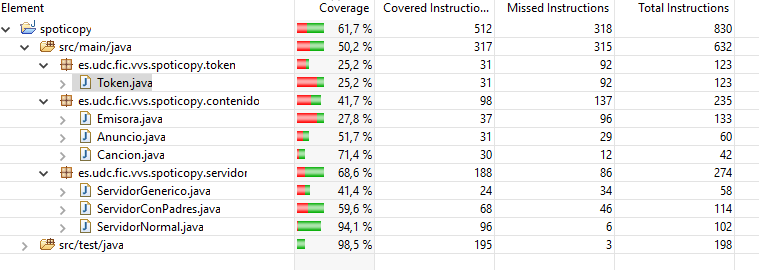
\includegraphics[width=15cm]{Imagenes/CoberturaSemana1.png} \\
	
	Después utilizar Junit para:
	\begin{itemize}
		\item Aumentar cobertura de Anuncio (casi al 100%)
		\item Aumentar cobertura de ServidorNormal (al 100%)
		\item Aumentar cobertura de ServidorGenerico (casi al 100%)
		\item Aumentar cobertura de Token 
		\item Aumentar cobertura de ServidorConPadres
	\end{itemize}
Quedó:
	
	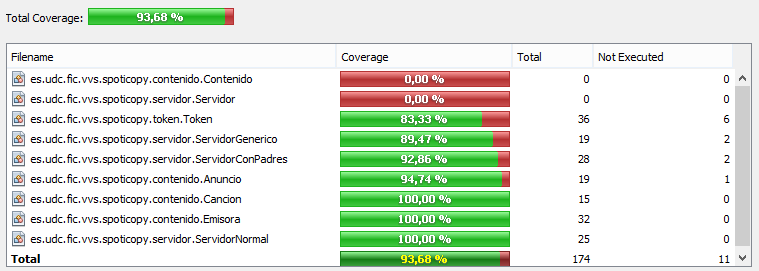
\includegraphics[width=15cm]{Imagenes/CoberturaSemana2.png} \\
	
	Después de realizar pruebas más exhautivas con junit y genenarlas con generadores a través de Quickcheck, de realizar pruebas de rendimiento con JETM, obtenemos mejores valores de cobertura:
	Resultado:
	
	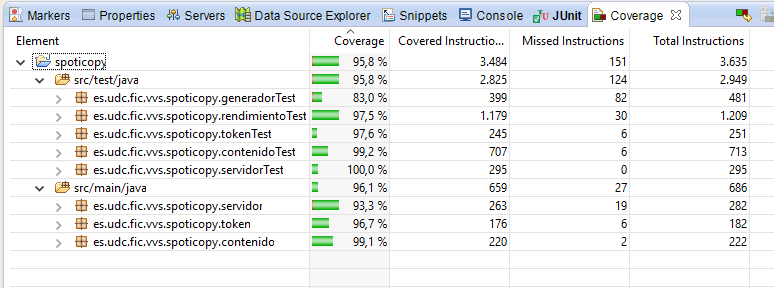
\includegraphics[width=15cm]{Imagenes/Covertura3.png} \\
	\subsection{PIT (mutation testing)}
	
	Realizado el mutation testing, resultados:
	
	\href{Informes/PIT1/index.html}{Informe PIT} \\
	
	\subsection{Pruebas estáticas/estructurales: FindBugs}
	
	FindBugs es un programa que utiliza el análisis estático para buscar errores en el código de Java.
	
	En la versión inicial podemos comprobar que tenemos los siguientes errores:
	\href{Informes/SiteTestInicial/findbugs.html}{Informe Find bugs} \\
	En el informe podemos comprobar que tenemos 9 bugs, y distinguimos dos categorías donde tenemos los problemas: Malas prácticas y problemas de estilo. También distinguimos la prioridad: Alta, baja y media.
	Los primeros errores a solventar son los de criticidad alta, seguidamente de los medios y por último los de prioridad baja.\\
	Errores encontrados:
		\begin{itemize}
			\item 	ST WRITE TO STATIC FROM INSTANCE METHOD: En la clase token existía un método que escribía en una variable estática, esto es una mala práctica cuando está siendo manipulado por varias instancias.
			\item 	RI REDUNDANT INTERFACES: ServidorNormal y ServidorConPadres implementa la misma interfaz que la superclase.
			\item BC EQUALS METHOD SHOULD WORK FOR ALL OBJECTS: El método equals (Object o) no debe hacer ninguna suposición sobre el tipo de o. Simplemente debe devolver false si o no es del mismo tipo que esta. La clase Anuncio asume el argumento es de tipo anuncio.
			\item HE EQUALS USE HASHCODE: La clase anuncio Esta clase anula Equals (Object) , pero no anula hashCode () , y hereda la implementación de hashCode () de java.lang.Object (que devuelve el código hash de identidad, un valor arbitrario asignado al objeto por el VM ) . Por lo tanto , es muy probable que violaría el invariante que los objetos iguales deben tener iguales hashcodes la clase.
			\item NP EQUALS SHOULD HANDLE NULL ARGUMENT: En la clase anuncio, el método no funciona para cuando el objeto es nulo.	
		\end{itemize}
		Después de identificar los errores, resolvedos los problemas mencionados y comprobamos el resultado:\\
		\\
	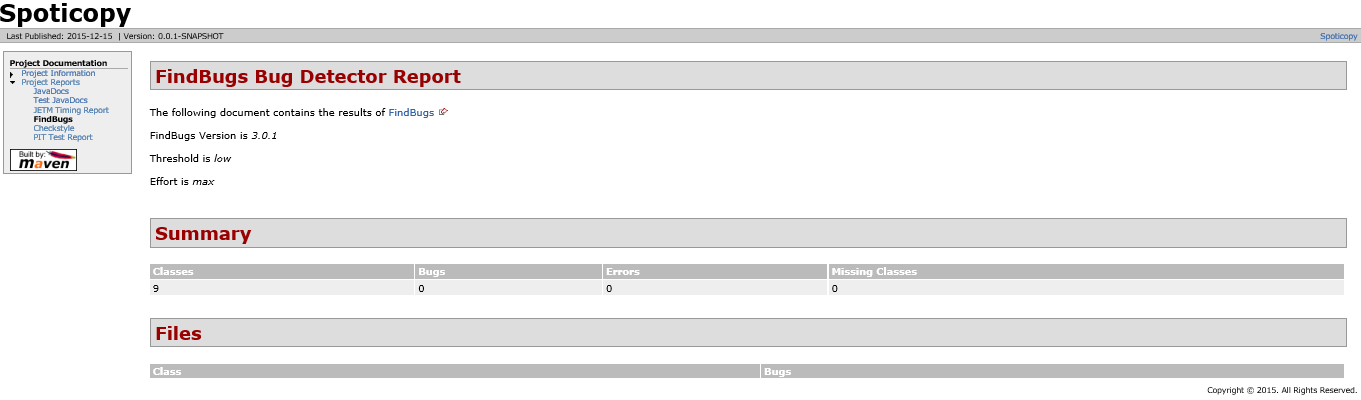
\includegraphics[width=15cm]{Imagenes/FindsBugs2.png} \\
	
		\subsection{Pruebas estáticas/estructurales: CheckStyle}
		
		Checkstyle es una herramienta de desarrollo para ayudar a los programadores escribir código Java que se adhiere a un estándar de codificación. 
		Para comprobar el estilo, pasamos la herramienta CheckStyle a nuestra aplicación y comprobamos el resultado:
		\href{Informes/SiteTestInicial/checkstyle.html}{Informe CheckStyle} \\
		Al pasar la herramienta de CheckStyle descubrimos que nuestra aplicación tiene unos 236 errores de estilo, es decir, que no cumple el estandar de programación java.
		
		Resumen de errores encontrados:
		\begin{itemize}
		\item Faltan comentarios: En la mayoría de clases faltan comentarios javadoc. Se añaden.
		\item Mala indexación código y espacios: Se reestructura el código para que solventar dichos errores.
		\end{itemize}
		
		Se revisa el informe con los 236 errores de estilo y se eliminan los 236 errores de estilo.
		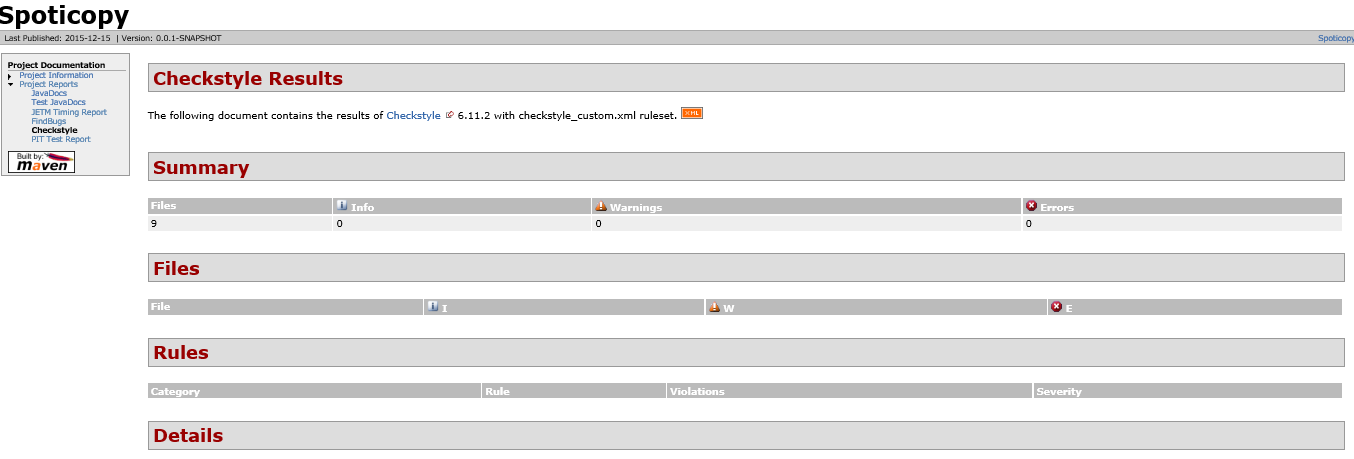
\includegraphics[width=15cm]{Imagenes/CheckStyleResut.png} \\
		
	\section{Registro de errores}
	
	Todos los errores localizados, modificaciones necesarias, etc. pueden encontrarse referenciados en el documento de CHANGELOG.txt, en el cual se encuentran las correcciones hasta el momento.
	
	\section{Estadísticas}
	
	\begin{itemize}
		\item Errores diarios encontrados:
		\item Errores semanales encontrados:
		\item Progreso en las pruebas:
		\item Análisis del perfil de detección de errores (lugares, componentes, tipología).
		\item Informe de errores abiertos y cerrados por nivel de criticidad.
		\item Evaluación global del estado de calidad y estabilidad actuales.
	\end{itemize}
	
	\section{Otros aspectos de interés}
	
	Nada de momento. Se conserva el apartado para el futuro.
	
\end{document}